\chapter{System Model and Methodology}
\begingroup
\justifying
\setlength{\parindent}{0pt}
\setstretch{1.5}
\setlength{\parskip}{0.5\baselineskip}
\titlespacing{\chapter}{0pt}{0pt}{0pt}
\titlespacing{\section}{0pt}{0pt}{0pt}

\section{Roles, Assets, and Trust Boundaries}

The protocol defines three active roles: administrator, registered voter, and public verifier. The main protected assets are ballot confidentiality, result correctness, and audit trace integrity.

Trust boundaries are split as follows:
\begin{itemize}
    \item \textbf{On-chain boundary}: election state transitions and proof-verification outcomes are publicly observable and tamper-evident.
    \item \textbf{Client boundary}: ballot construction, witness generation, and receipt storage occur in user-controlled runtime environments.
    \item \textbf{Administrator boundary}: tally decryption key custody and result submission remain operationally sensitive.
\end{itemize}

\section{Threat Model}

The model considers malicious voters, passive blockchain observers, and potentially faulty administrators. The following attacks are explicitly targeted:
\begin{itemize}
    \item invalid ballot shape (non-one-hot encryption);
    \item out-of-range candidate encoding;
    \item replay or duplicate voting attempts;
    \item fabricated tally claims unsupported by valid proof.
\end{itemize}

The following are not fully solved in the current prototype: coercion resistance, malware-compromised browser clients, and threshold key governance.

\section{Protocol State Machine}

Election lifecycle states are:
\begin{equation}
S = \{\texttt{Created},\ \texttt{Active},\ \texttt{Ended},\ \texttt{Tallied}\}
\end{equation}

Allowed transitions are:
\begin{equation}
\texttt{Created} \rightarrow \texttt{Active} \rightarrow \texttt{Ended} \rightarrow \texttt{Tallied}
\end{equation}

This deterministic state machine ensures that vote submission only occurs in the active phase and tally finalization only occurs after the election is ended.

Figure \ref{fig:protocol-flow} summarizes the complete interaction sequence among administrator, voters, and smart contracts.

\begin{figure}[htbp]
\centering
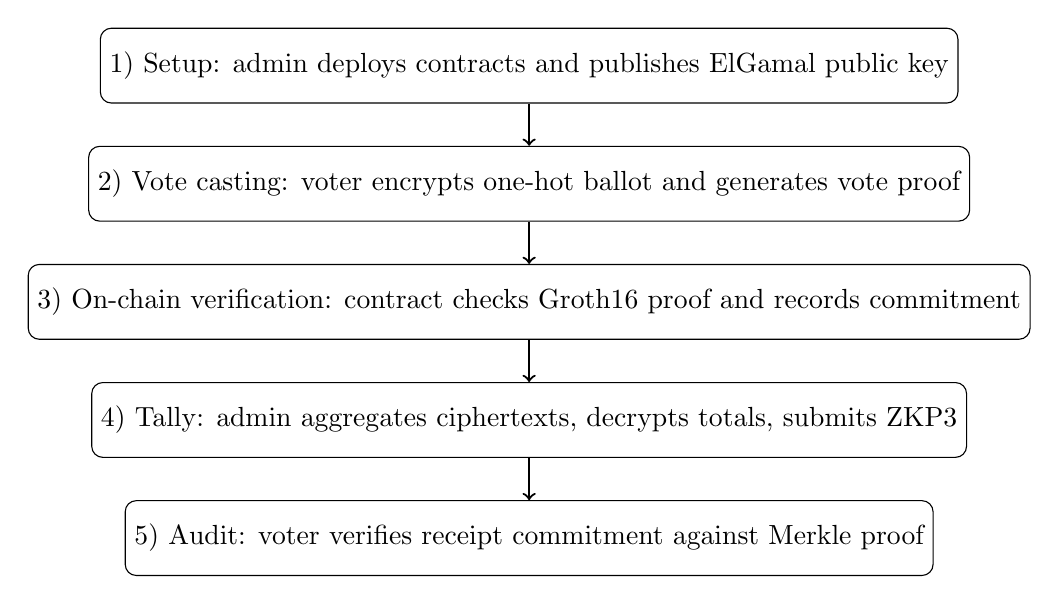
\begin{tikzpicture}[x=1cm,y=1cm]
    \node[draw, rounded corners, minimum width=8.6cm, minimum height=0.95cm] (a) at (0,0) {1) Setup: admin deploys contracts and publishes ElGamal public key};
    \node[draw, rounded corners, minimum width=8.6cm, minimum height=0.95cm] (b) at (0,-1.5) {2) Vote casting: voter encrypts one-hot ballot and generates vote proof};
    \node[draw, rounded corners, minimum width=8.6cm, minimum height=0.95cm] (c) at (0,-3.0) {3) On-chain verification: contract checks Groth16 proof and records commitment};
    \node[draw, rounded corners, minimum width=8.6cm, minimum height=0.95cm] (d) at (0,-4.5) {4) Tally: admin aggregates ciphertexts, decrypts totals, submits ZKP3};
    \node[draw, rounded corners, minimum width=8.6cm, minimum height=0.95cm] (e) at (0,-6.0) {5) Audit: voter verifies receipt commitment against Merkle proof};

    \draw[->, thick] (a) -- (b);
    \draw[->, thick] (b) -- (c);
    \draw[->, thick] (c) -- (d);
    \draw[->, thick] (d) -- (e);
\end{tikzpicture}
\caption{End-to-End Protocol Flow}
\label{fig:protocol-flow}
\end{figure}

Figure \ref{fig:protocol-sequence} provides a sequence-style view of the same workflow with explicit message directions.

\begin{figure}[htbp]
\centering
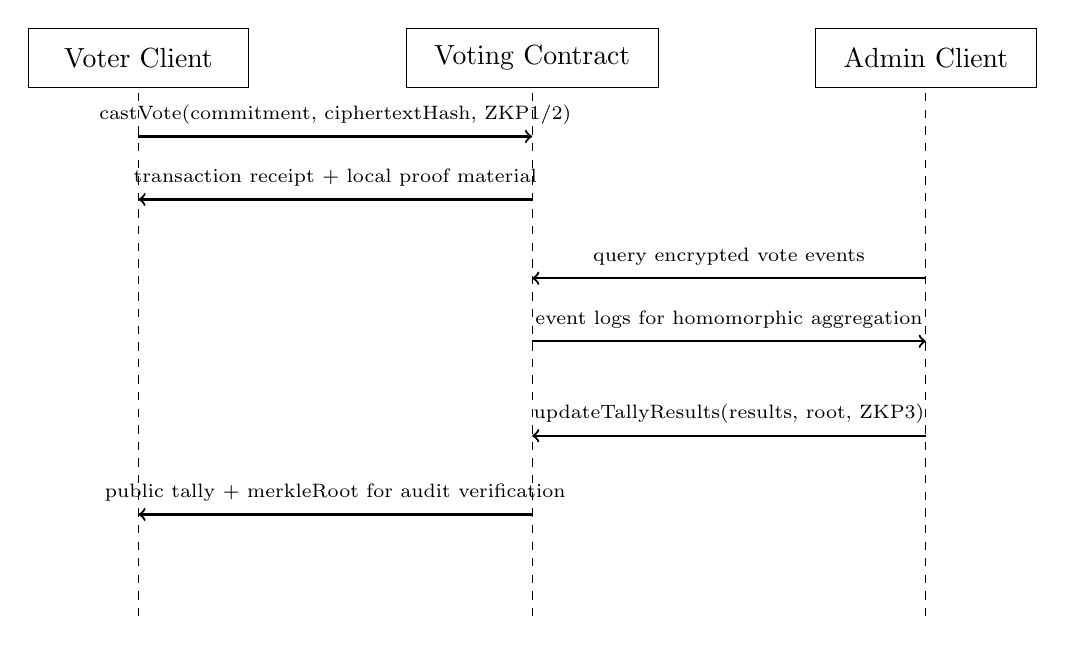
\begin{tikzpicture}[x=1cm,y=1cm]
    \node[draw, minimum width=2.8cm, minimum height=0.75cm] (voter) at (0,0) {Voter Client};
    \node[draw, minimum width=3.2cm, minimum height=0.75cm] (chain) at (5.0,0) {Voting Contract};
    \node[draw, minimum width=2.8cm, minimum height=0.75cm] (admin) at (10.0,0) {Admin Client};

    \draw[dashed] (0,-0.45) -- (0,-7.1);
    \draw[dashed] (5.0,-0.45) -- (5.0,-7.1);
    \draw[dashed] (10.0,-0.45) -- (10.0,-7.1);

    \draw[->, thick] (0,-1.0) -- (5.0,-1.0);
    \node[font=\scriptsize, align=center] at (2.5,-0.72) {castVote(commitment, ciphertextHash, ZKP1/2)};

    \draw[->, thick] (5.0,-1.8) -- (0,-1.8);
    \node[font=\scriptsize, align=center] at (2.5,-1.52) {transaction receipt + local proof material};

    \draw[->, thick] (10.0,-2.8) -- (5.0,-2.8);
    \node[font=\scriptsize, align=center] at (7.5,-2.52) {query encrypted vote events};

    \draw[->, thick] (5.0,-3.6) -- (10.0,-3.6);
    \node[font=\scriptsize, align=center] at (7.5,-3.32) {event logs for homomorphic aggregation};

    \draw[->, thick] (10.0,-4.8) -- (5.0,-4.8);
    \node[font=\scriptsize, align=center] at (7.5,-4.52) {updateTallyResults(results, root, ZKP3)};

    \draw[->, thick] (5.0,-5.8) -- (0,-5.8);
    \node[font=\scriptsize, align=center] at (2.5,-5.52) {public tally + merkleRoot for audit verification};
\end{tikzpicture}
\caption{Protocol Sequence Diagram for Voting and Tally}
\label{fig:protocol-sequence}
\end{figure}

\section{Ballot Encoding and Encryption}

Let $N$ be the number of candidates and $v \in \{0,1,\dots,N-1\}$ be the selected candidate index. A ballot is encoded as one-hot vector
$\mathbf{m}=(m_0,\dots,m_{N-1})$ where $m_v=1$ and all other entries are $0$.

For each position $i$, ElGamal ciphertext is generated on BabyJubJub:
\begin{equation}
C1_i = r_i \cdot G, \quad C2_i = m_i \cdot G + r_i \cdot \mathit{PK}
\end{equation}
where $r_i$ is random nonce, $G$ is generator, and $\mathit{PK}$ is administrator public key.

\section{Commitment and Ciphertext Binding}

For random salt $s$, commitment is defined as:
\begin{equation}
\mathit{Com} = \mathsf{Poseidon}(v,\, s)
\end{equation}

Ciphertext binding hash is defined over all ciphertext coordinates:
\begin{equation}
\begin{split}
H_{ct} = \mathsf{Poseidon}(&\mathit{c1X}_0,\,\mathit{c1Y}_0,\,\mathit{c2X}_0,\,\mathit{c2Y}_0,\,\dots,\\
                  &\mathit{c1X}_{N-1},\,\mathit{c1Y}_{N-1},\,\mathit{c2X}_{N-1},\,\mathit{c2Y}_{N-1})
\end{split}
\end{equation}

The vote proof uses $(\mathit{Com}, H_{ct}, pk_X, pk_Y)$ as public signals and proves consistency between commitment, candidate index, and encrypted one-hot structure.

\section{Vote Proof Constraints}

The vote circuit enforces four constraint families:
\begin{enumerate}
    \item \textbf{Commitment consistency}: public commitment equals Poseidon of private candidate index and salt.
    \item \textbf{Range check}: candidate index is strictly less than configured candidate cardinality.
    \item \textbf{One-hot encryption validity}: encrypted slot equals 1 for selected index and 0 otherwise.
    \item \textbf{Ciphertext binding}: public ciphertext hash equals Poseidon hash of all ciphertext components.
\end{enumerate}

This composition ensures that an accepted vote is both syntactically and semantically valid under protocol rules.

\section{Homomorphic Tally and Tally Proof}

For each candidate position $j$, aggregated ciphertext is computed by point addition across all votes:
\begin{equation}
\bar{C1}_j = \sum_{k=1}^{V} C1_{k,j}, \quad \bar{C2}_j = \sum_{k=1}^{V} C2_{k,j}
\end{equation}

Given secret key $sk$, decryption result point is:
\begin{equation}
R_j = \bar{C2}_j - sk \cdot \bar{C1}_j
\end{equation}

The tally circuit proves:
\begin{itemize}
    \item key ownership consistency: $\mathit{PK} = sk \cdot G$;
    \item decryption correctness per candidate;
    \item sum consistency of all result points with total vote count.
\end{itemize}

\section{Merkle Audit Construction}

The audit set uses commitment values as leaves directly:
\begin{equation}
\mathit{leaf}_i = \mathit{commitment}_i
\end{equation}

Internal nodes are built using Keccak over ordered child pair:
\begin{equation}
\mathit{node} = \mathsf{keccak256}(\mathit{left} \parallel \mathit{right})
\end{equation}

If a layer has odd cardinality, the last node is duplicated. Commitments are sorted by
\texttt{blockNumber}, \texttt{transactionIndex}, and \texttt{logIndex} before tree construction to guarantee deterministic roots.

\section{Anonymous Verification Procedure}

A voter stores local receipt fields: candidate ID, salt, commitment, transaction hash, and election ID.
Verification executes:
\begin{enumerate}
    \item recompute commitment from candidate ID and salt;
    \item locate matching commitment entry in audit bundle;
    \item verify Merkle path to bundle root;
    \item accept if and only if proof is valid and election metadata matches.
\end{enumerate}

This procedure allows individual inclusion checks without exposing wallet address linkage.

Table \ref{tab:audit-artifacts} lists the main artifacts that participate in anonymous verification.

\begin{table}[htbp]
\centering
\small
\caption{Audit Artifacts and Their Roles}
\label{tab:audit-artifacts}
\begin{tabular}{L{3.2cm} L{3.8cm} L{5.8cm}}
\toprule
Artifact & Source & Verification Role \\
\midrule
Receipt JSON & Voter local storage & Provides candidate ID, salt, and commitment to recompute commitment consistency. \\
Commitment leaf & On-chain vote event & Represents one ballot commitment in Merkle construction. \\
Proof path & Audit bundle entry & Enables logarithmic-size inclusion verification against bundle root. \\
Merkle root & Tally publication / bundle metadata & Serves as commitment set digest to validate inclusion outcome. \\
Election ID & Bundle + receipt metadata & Prevents cross-election replay or accidental bundle mismatch. \\
\bottomrule
\end{tabular}
\end{table}

\section{Complexity and Scalability Considerations}

For $V$ votes and $N$ candidates:
\begin{itemize}
    \item ballot encryption complexity is $O(N)$ per voter;
    \item tally aggregation complexity is $O(VN)$ point additions;
    \item single inclusion proof verification is $O(\log V)$ hash operations.
\end{itemize}

While the current implementation is suitable for small-to-medium election sizes in prototype settings, larger deployments require optimization of proof generation latency, event indexing, and key governance.

\section{Chapter Summary}

This chapter formalized the protocol model, specified threat assumptions, and defined the cryptographic workflow from ballot encoding to anonymous audit verification. It also established deterministic Merkle construction rules and complexity bounds that guide the implementation choices described in Chapter 4. Where this chapter specified \emph{what} the protocol must do, Chapter 4 describes \emph{how} each component is realized in code, and the specific engineering decisions taken at each layer.

\endgroup

